\documentclass{article}\usepackage[]{graphicx}\usepackage[]{color}
%% maxwidth is the original width if it is less than linewidth
%% otherwise use linewidth (to make sure the graphics do not exceed the margin)
\makeatletter
\def\maxwidth{ %
  \ifdim\Gin@nat@width>\linewidth
    \linewidth
  \else
    \Gin@nat@width
  \fi
}
\makeatother

\definecolor{fgcolor}{rgb}{0.345, 0.345, 0.345}
\newcommand{\hlnum}[1]{\textcolor[rgb]{0.686,0.059,0.569}{#1}}%
\newcommand{\hlstr}[1]{\textcolor[rgb]{0.192,0.494,0.8}{#1}}%
\newcommand{\hlcom}[1]{\textcolor[rgb]{0.678,0.584,0.686}{\textit{#1}}}%
\newcommand{\hlopt}[1]{\textcolor[rgb]{0,0,0}{#1}}%
\newcommand{\hlstd}[1]{\textcolor[rgb]{0.345,0.345,0.345}{#1}}%
\newcommand{\hlkwa}[1]{\textcolor[rgb]{0.161,0.373,0.58}{\textbf{#1}}}%
\newcommand{\hlkwb}[1]{\textcolor[rgb]{0.69,0.353,0.396}{#1}}%
\newcommand{\hlkwc}[1]{\textcolor[rgb]{0.333,0.667,0.333}{#1}}%
\newcommand{\hlkwd}[1]{\textcolor[rgb]{0.737,0.353,0.396}{\textbf{#1}}}%
\let\hlipl\hlkwb

\usepackage{framed}
\makeatletter
\newenvironment{kframe}{%
 \def\at@end@of@kframe{}%
 \ifinner\ifhmode%
  \def\at@end@of@kframe{\end{minipage}}%
  \begin{minipage}{\columnwidth}%
 \fi\fi%
 \def\FrameCommand##1{\hskip\@totalleftmargin \hskip-\fboxsep
 \colorbox{shadecolor}{##1}\hskip-\fboxsep
     % There is no \\@totalrightmargin, so:
     \hskip-\linewidth \hskip-\@totalleftmargin \hskip\columnwidth}%
 \MakeFramed {\advance\hsize-\width
   \@totalleftmargin\z@ \linewidth\hsize
   \@setminipage}}%
 {\par\unskip\endMakeFramed%
 \at@end@of@kframe}
\makeatother

\definecolor{shadecolor}{rgb}{.97, .97, .97}
\definecolor{messagecolor}{rgb}{0, 0, 0}
\definecolor{warningcolor}{rgb}{1, 0, 1}
\definecolor{errorcolor}{rgb}{1, 0, 0}
\newenvironment{knitrout}{}{} % an empty environment to be redefined in TeX

\usepackage{alltt}

\title{STAT 243 Final Group Project}
\author{
  Dongyu Lang
  \and
  Amanda Mok
  \and
  Kehsin Su
  \and
  Junyi Tang
}
\IfFileExists{upquote.sty}{\usepackage{upquote}}{}
\begin{document}

\maketitle

The final version of the project resides at \texttt{https://github.com/amandamok/GA}

\section{Solution description}

This GA package primarily works on objects of two classes: \texttt{chromosome} and \texttt{population}. Objects of class \texttt{chromosome} contain a vector of 0's and 1's indicating a predictor's inclusion in a linear model, as well as the associated fitness (defaults to AIC) of that model. Objects of class \texttt{population} contain the original data (with the response variable as the first column), a list of \texttt{chromosome} objects that represent the models in the population at that generation, and the model with the best fitness out of that generation's population.

The following functions perform operations at the chromosome level. \texttt{initChrom()} initializes an object of class \texttt{chromosome}; if the variable inclusion vector is not provided, then the function will provide a random vector of 0's and 1's. \texttt{convertFormula()} will translate that vector into a formula object for input into \texttt{glm()}. \texttt{evalFitness()} will return the "fitness" (defaults to AIC, but can handle other functions that operate on \texttt{glm} objects) of a chromosome. \texttt{mutateChrom} will convert 0's to 1's and 1's to 0's at some probability \texttt{pMutate} at each locus on a single chromosome.

The following functions perform operations at the population level. \texttt{getFitness()} retrieves the fitness scores for a population of \texttt{chromosome} objects. \texttt{crossover()} takes two \texttt{chromosomes} and induces a "crossover" event at a random locus, producing a single offspring model. \texttt{mutatePop()} performs mutations (as dictated by \texttt{mutateChrom} at the population level. The function \texttt{nextGen} performs all the steps of each generation/iteration: removing the \texttt{pSelect}*100\% models with the lowest fitness, repopulating with new \texttt{chromosome} objects using \texttt{crossover()}, and randomly performing mutations on all \texttt{chromosomes} in the population with \texttt{mutatePop()}.

Finally, a wrapper function \texttt{select()} initializes the population and performs the genetic algorithm, given user-supplied data (with the user supplying the name of the response variable), size of the population at each generation \texttt{popSize}, the proportion of the population to select off at each generation \texttt{pSelect}, the probability of mutation at an individual locus on an individual chromosome \texttt{pMutate}, the number of iterations to run the genetic algorithm \texttt{max\_iter}, the fitness function to minimize \texttt{fitfunc}, and the \texttt{family} parameter to input into \texttt{glm()}. The wrapper function returns the a list with the formula, variable inclusion vector, and associated fitness of the best model after all the iterations; it also plots the best fitness and the average fitness across the population per generation.

\section{Testing}

Each function in the package is tested if the output is of the correct class. When appropriate, the function is tested for when the user provides the incorrect input. If the function provides a consistent result (i.e. \texttt{evalFitness} and \texttt{convertFormula}), the output of the function is compared to results if another method was used.

\section{Example implementation}

\begin{knitrout}
\definecolor{shadecolor}{rgb}{0.969, 0.969, 0.969}\color{fgcolor}\begin{kframe}
\begin{alltt}
\hlstd{devtools}\hlopt{::}\hlkwd{install_github}\hlstd{(}\hlkwd{paste0}\hlstd{(}\hlstr{"amandamok"}\hlstd{,} \hlstr{"/GA"}\hlstd{),} \hlkwc{force}\hlstd{=T)}
\end{alltt}


{\ttfamily\noindent\color{warningcolor}{\#\# Warning in strptime(x, fmt, tz = "{}GMT"{}): unknown timezone 'default/America/Los\_Angeles'}}

{\ttfamily\noindent\itshape\color{messagecolor}{\#\# Downloading GitHub repo amandamok/GA@master\\\#\# from URL https://api.github.com/repos/amandamok/GA/zipball/master}}

{\ttfamily\noindent\itshape\color{messagecolor}{\#\# Installing GA}}

{\ttfamily\noindent\itshape\color{messagecolor}{\#\# '/Library/Frameworks/R.framework/Resources/bin/R' --no-site-file\ \ \textbackslash{}\\\#\#\ \  --no-environ --no-save --no-restore --quiet CMD INSTALL\ \ \textbackslash{}\\\#\#\ \  '/private/var/folders/n2/f\_58kj8x371d4syzjrhvlk1m0000gn/T/Rtmp2rmamw/devtools11cf5ae1b0ac/amandamok-GA-dc517eb'\ \ \textbackslash{}\\\#\#\ \  --library='/Users/pandagoneamok/Library/R/3.4/library' --install-tests}}

{\ttfamily\noindent\itshape\color{messagecolor}{\#\# }}

{\ttfamily\noindent\itshape\color{messagecolor}{\#\# Reloading installed GA}}\begin{alltt}
\hlkwd{library}\hlstd{(GA)}

\hlkwd{set.seed}\hlstd{(}\hlnum{1}\hlstd{)}
\hlstd{results} \hlkwb{=} \hlkwd{select}\hlstd{(mtcars,} \hlstr{"mpg"}\hlstd{,} \hlkwc{popSize}\hlstd{=}\hlnum{50}\hlstd{)}
\end{alltt}
\begin{verbatim}
## [1] "Finished the 100th iteration."
## [1] "Finished the 200th iteration."
## [1] "Finished the 300th iteration."
## [1] "Finished the 400th iteration."
## [1] "Finished the 500th iteration."
## [1] "Finished the 600th iteration."
## [1] "Finished the 700th iteration."
## [1] "Finished the 800th iteration."
## [1] "Finished the 900th iteration."
## [1] "Finished the 1000th iteration."
## [1] "This select function reaches the number of maximum iterations.The best model selected by AIC using gaussian distribution within the maximum iterations has the fitness value as 155.476628510258."
\end{verbatim}
\end{kframe}
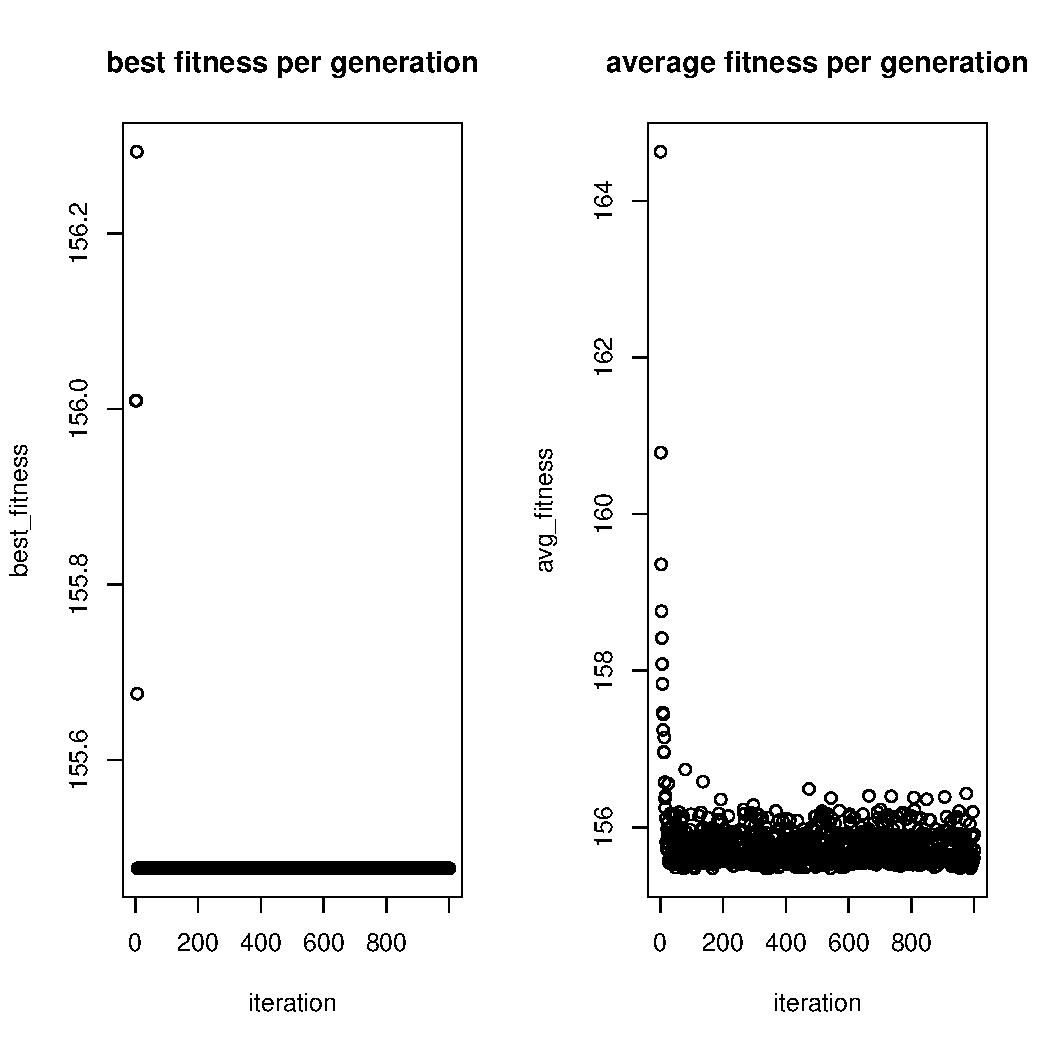
\includegraphics[width=\maxwidth]{figure/unnamed-chunk-1-1} 
\begin{kframe}\begin{alltt}
\hlstd{results}\hlopt{$}\hlstd{model}
\end{alltt}
\begin{verbatim}
## [1] "mpg  ~  cyl + hp + wt"
\end{verbatim}
\begin{alltt}
\hlstd{results}\hlopt{$}\hlstd{fitness}
\end{alltt}
\begin{verbatim}
## [1] 155.4766
\end{verbatim}
\end{kframe}
\end{knitrout}

\section{Contributions}

Group members contributed to the final project as follows:

Dongyu Lang: package tests (initialization)

Amanda Mok: helper functions that operate on \texttt{chromosome} and \texttt{population} objects; project write-up (mutation, crossover)

Kehsin Su: package documentation (model selection)

Junyi Tang: wrapper function and plotting of results (write up and function wrap up)\\

Note: parentheses is the original part of works. Considering consistency and the efficiency, we finally used Ameanda's version, but all the members have written up their functions at the beginning.
\end{document}
